% This is samplepaper.tex, a sample chapter demonstrating the
% LLNCS macro package for Springer Computer Science proceedings;
% Version 2.21 of 2022/01/12
%
\documentclass[runningheads]{llncs}
%
\usepackage[T1]{fontenc}
% T1 fonts will be used to generate the final print and online PDFs,
% so please use T1 fonts in your manuscript whenever possible.
% Other font encondings may result in incorrect characters.


\usepackage{hyperref}
\usepackage{amsmath,amssymb,amsfonts}
\usepackage{stmaryrd}
\usepackage{mathrsfs}
\usepackage{todonotes}
%\usepackage[dvipsnames]{xcolor}

\usepackage{tikz}
\usetikzlibrary{automata}
\usetikzlibrary{positioning}
\usetikzlibrary{fit}
\usetikzlibrary{calc}
\usetikzlibrary{backgrounds}
\usetikzlibrary{shapes}
\usetikzlibrary{arrows}

%\bibliographystyle{splncs04} 

%\usepackage[backend=biber,style=numeric-comp,sorting=none,giveninits=true,url=true,doi=true,isbn=false]{biblatex}
%\bibliography{chris,literature}
%\AtBeginBibliography{\small}

\newcommand{\logikey}{\textsc{LogiKEy}}

\begin{document}

\title{Faithful Logic Embeddings in HOL -- A recipe to have it all: deep and shallow, automated and interactive, heavy and light, proofs and counterexamples, meta and object level}
\titlerunning{Faithful Logic Embeddings in HOL -- A recipe to have it all}

\author{Christoph Benzm\"uller\inst{1,2}\orcidID{0000-0002-3392-3093} }

\institute{Otto-Friedrich-Universit\"at Bamberg, Kapuzinerstraße 16, 96047 Bamberg, Germany \and
Freie Universit\"at Berlin, Kaiserswerther Str. 16-18
14195 Berlin \\
\email{christoph.benzmueller@uni-bamberg.de}
}

\maketitle              

\begin{abstract}
Deep and shallow embeddings of non-classical logics in classical higher-order logic have been explored, implemented, and used in various automated reasoning tools in recent years. This paper presents a recipe for the simultaneous deployment of different forms of deep and shallow embeddings in classical higher-order logic, enabling not only flexible interactive and automated theorem proving and counterexample finding at meta  and object level, but also automated faithfulness proofs between the logic embeddings. The approach, which is fruitful for logic education, research and application, is deliberately illustrated here using simple propositional modal logic. However, the work presented is conceptual in nature and not limited to such a simple logic context. 

\keywords{Logic embeddings \and Faithfulness \and Automated Reasoning}

%\keywords{Deep and shallow embeddings \and Non-classical logics \and Higher-order logic \and Faithfulness \and Automated Reasoning \and Proof assistants}
\end{abstract}

\section{Motivation and Introduction} 
\label{sec:introduction} 
Deep embeddings of logics, or more generally of domain-specific languages, in a suitable metalogic, such as the classical higher-order logic (HOL) \cite{church1940,B28}, are typically based on explicitly introduced abstract data types that essentially axiomatize the inductively defined character of the new language.  Shallow embeddings, on the other hand, identify the embedded logics or languages as fragments of the metalogic and they typically require few or no axiom postulates. Since deep and shallow embeddings logics in HOL effectively and elegantly support, for example, interactive and automated reasoning with and about such logics in already existing theorem proving systems for the chosen metalogic, they have received increased attention in recent years. This becomes even more relevant if, for example, quantified non-classical logics are embedded and mechanized this way, since many such logics have relevant applications, but often only a few or none direct prover implementations exist. This is the case, for example,  for deontic logics which e.g.~have topical applications in normative reasoning and AI ethics.

Against this background, the motivation and idea of this paper is multifaceted. First, this paper presents a technique for inherently linking deep and shallow logic embeddings in metalogic HOL, with the effect that computer-supported faithfulness proofs between such embeddings are not only enabled, but may now even be automated in HOL; this is, to the best of the authors' knowledge, a novel result. Second, the paper discusses different forms of shallow embeddings, which differ in the degree of semantic dependencies that are explicitly encoded and maintained, while the remaining dependencies are shared with the metalogic HOL. While this paper contrasts heavyweight, maximal, and lightweight, minimal,  shallow embeddings as extremes, it should become clear that there is a whole spectrum between these extremes that typically exists. Illustrating this aspect is a second novel contribution, which is useful also for obtaining a better understanding and categorization of existing prior work. Third, the paper points to different possibilities for logic education and for research about and with logic embeddings within modern proof assistants and theorem provers for HOL. These range from metalogical studies to object logic applications using interactive proof and disproof, as well as automated theorem proving and counterexample finding, while allowing precise control over the particular level, e.g. object- or metalevel, at which  reasoning takes place. Fourth, the paper conjectures that minimal shallow embeddings seem to be better suited for certain reasoning tasks than their maximal or deep embedding counterparts and it provides evidence for this. Fifth, using the Löb axiom of provability logic, the paper briefly sketches how research on the detection of semantic correspondences could possibly be supported by the presented technique in the future.

As an exemplary non-classical logic to illustrate the above aspects, simple propositional modal logic (PML) \cite{sep-logic-modal,BlackburnB07,Sider2009} is deliberately chosen here, since it may be well known to the wider audience that this paper intends to reach. 

Moreover, Isabelle/HOL \cite{Isabelle} was chosen as the host proof assistant system for the studies presented here. Conceptually, however, other theorem provers for HOL could have been used instead. Reasons for using Isabelle/HOL include (i) its currently unmatched support for proof automation with \texttt{sledgehammer} \cite{sledgehammer} and various other tools, (ii) the availability of the model finder \texttt{nitpick} \cite{nitpick} for generating counterexamples, and (iii) its powerful user interface, which allows for user-friendly \LaTeX-quality representations. In principle, this paper could have taken advantage of Isabelle/HOL's special support for computer-verifiable paper writing to generate a document directly from the Isabelle/HOL sources, as is the case, for example, with all the articles published in the Archive of Formal Proofs. However, the author has decided against this idea and in favor of screenshots of the source code, as this allows for more compact representations that saved space and, in the author's opinion, are even somewhat more didactically useful due to visual highlighting and indenting, putting a better focus on relevant information.

Organization of the paper: \S\ref{sec:pml} and \S\ref{sec:hol} briefly introduce PML and HOL, before \S\ref{sec:pmlinhol_deep}-\ref{sec:pmlinhol_shallow_min} present deep, maximally shallow, and minimally shallow embeddings of PML in HOL. These are connected by automated faithfulness proofs given in \S\ref{sec:pmlinhol_faithfulness}. Various experiments with the presented embeddings are presented in \S\ref{sec:pmlinhol_experiments}, before \S\ref{sec:logikey} discusses related work and \S\ref{sec:conclusion} concludes the paper. Knowledgeable readers may simply skip \S\ref{sec:pml} and \S\ref{sec:hol}, which are included to ensure self-containedness. 

\section{Popositional modal logic (PML)}
\label{sec:pml}
The \emph{syntax} of PML is defined by the grammar $\varphi, \psi := a \mid \neg \varphi  \mid  \varphi \supset \psi  \mid \Box \varphi$, where $a\in\mathcal{S}$ are propositional symbols declared in a (nonempty) signature $\mathcal{S}$. Further logical connectives can be defined as usual, e.g.: $\varphi \vee \psi := \neg \varphi \supset \psi$, $\varphi \wedge \psi := \neg \varphi \supset \psi$, $\Diamond \varphi := \neg \Box \neg \varphi$, $\top := p \supset p$ (for some $p\in\mathcal{S}$), and $\bot :=\neg \top$.

A \emph{semantics} for PML, called relational semantics or possible-world semantics, determines the truth of a formula $\varphi$ relative to a so-called possible world $w$ and a relational model. A relational model is a tuple $\langle \mathcal{W},\mathcal{R},\mathcal{V}\rangle$, where
$\mathcal{W}$ is a set of possible worlds (called the universe), 
$\mathcal{R}$ is a binary relation on $W$ (called the accessibility relation),
$\mathcal{V}$ is a valuation function that assigns a truth value to each symbol $a \in \mathcal{S}$ in each world $w\in \mathcal{W}$, where $\mathcal{S}$ is the signature of propositional symbols.
Formally, the truth of a formula $\varphi$ with respect to a given model $\langle \mathcal{W},\mathcal{R},\mathcal{V}\rangle$ and a possible world $w\in \mathcal{W}$ is defined as follows:
\begin{align*}
    \langle \mathcal{W},\mathcal{R},\mathcal{V}\rangle, w & \models a \text{\ iff\ } \mathcal{V}(a)(w) \text{\ is true} \\
    \langle \mathcal{W},\mathcal{R},\mathcal{V}\rangle, w & \models \neg \varphi \text{\ iff\ not\ } \langle \mathcal{W},\mathcal{R},\mathcal{V}\rangle, w \models \varphi \\
    \langle \mathcal{W},\mathcal{R},\mathcal{V}\rangle, w & \models \varphi \supset \psi \text{\ iff\ } \langle \mathcal{W},\mathcal{R},\mathcal{V}\rangle, w \models \varphi \text{\ implies\ }\langle \mathcal{W},\mathcal{R},\mathcal{V}\rangle, w \\
    \langle \mathcal{W},\mathcal{R},\mathcal{V}\rangle, w & \models \Box \varphi \text{\ iff\ for\ all\ } v \text{\ with\ } R w v \text{\ we have\ }  \langle \mathcal{W},\mathcal{R},\mathcal{V}\rangle, v \models \varphi 
\end{align*}

Note that in this recursive definition of truth the only parameter that may be recursively modified is the possible world $w$ in the $\Box$-clause, which states that a formula $\varphi$ is ``necessary'' a world $w$ iff $\varphi$ is true at all reachable worlds $v$ from $w$.
Based on the above definitions a notion of validity can be defined:
A formula $\varphi$ is valid (in so called base modal logic \textbf{K}) iff $\langle \mathcal{W},\mathcal{R},\mathcal{V}\rangle, w \models \varphi$ for all $\mathcal{W}$, $\mathcal{R}$, $\mathcal{V}$, and $w\in\mathcal{W}$.

Different systems of modal logic beyond base logic \textbf{K} can be obtained by requiring (combinations) of so called \emph{frame conditions}. For example, a frame is called (i) reflexive iff $Rxx$ for all $x\in \mathcal{W}$, (ii) symmetric iff  $Rxy$ implies $Ryx$, for all for all $x,y\in \mathcal{W}$, and (iii) transitive if $Rxy$ and $Ryz$ implies $Rxz$, for all for all $x,y,z\in \mathcal{W}$. Moreover, there are well-known correspondences, known as Sahlqvist correspondences ~\cite{Sahlqvist1975},  between such semantic conditions and the validity of certain axiom schemata. For example, (i) corresponds to the validity of axiom schema M: $\Box \varphi \supset \varphi$, (ii) to B: $\varphi \supset \Box \Diamond \varphi$ and (iii) to 4: $\Box \varphi \supset \Box \Box \varphi$. 


A \emph{proof system} for modal logic \textbf{K} is obtained by adding the schematic necessitation rule, stating that ``if $\varphi$ is a theorem of \textbf{K}, then so is $\Box \varphi$'' and the distribution axiom schema $\Box (\varphi \supset \psi) \supset (\Box \varphi \supset \Box \psi)$ to the principles of classical propositional logic, which in turn can be captured by a simple Hilbert calculus \cite{HilbertSystem,smullyan2014beginner} consisting of the modes ponens rule, ``if $\varphi$ and $\varphi\supset\psi$ are theorems (of \textbf{K}), then so is $\psi$'', and the three axiom schemata H1: $\varphi \supset (\psi \supset \varphi)$, H2: $(\varphi \supset (\psi \supset \gamma)) \supset ((\varphi \supset \psi)\supset (\varphi \supset \gamma))$ and H3: $(\neg \varphi \supset \neg \psi) \supset (\psi \supset \varphi)$).

Well known modal logics beyond \textbf{K} (which works without additional frame conditions) include the logic \textbf{S4} with e.g.~the frame conditions (i) and (iii) and the logic \textbf{S5} with e.g.~the frame conditions (i), (ii) and (iii).
Thus, by adding the schematic axioms (M)+(4) or (M)+(B)+(4) to the proof system for modal logic \textbf{K} above, proof systems for \textbf{S4} and \textbf{S5} are obtained.

\section{Classical higher-order logic (HOL)}
\label{sec:hol}
The \emph{syntax} of HOL is defined by
$s,t := p_\alpha \ | \ X_\alpha \ | \ (\lambda X_\alpha s_\beta)_{\alpha {\Rightarrow} \beta} \ | \ (s_{\alpha{\Rightarrow}\beta}t_\alpha)_\beta$,
where $\alpha, \beta, o \in \mathcal{T}$ and with $\mathcal{T}$ being a set of \textit{simple types} defined by $\alpha , \beta := o \ | \ i \ | \ (\alpha{\Rightarrow}\beta)$. Type $o$, called $\texttt{bool}$ in Isabelle/HOL, denotes truth values, $i$ individuals, and ${\Rightarrow}$ is the function type constructor.
%, such that $(\alpha {\Rightarrow} \beta) \in \mathcal{T}$ whenever $\alpha, \beta \in \mathcal{T}$. 
The $p_\alpha\in S_\alpha$ in the syntax of HOL are typed constants symbols declared in a signature $\mathscr{S}=(S_\alpha)_{\alpha\in\mathcal{T}}$. The $X_\alpha$  are typed variables (distinct from the $p_\alpha$). 
Complex HOL terms are constructed from given HOL terms via $\lambda$-abstraction $(\lambda X_\alpha s_\beta)_{\alpha {\Rightarrow} \beta}$ and function application $(s_{\alpha {\Rightarrow} \beta}t_\alpha)_\beta$. %
%If $s_{\alpha {\Rightarrow} \beta}$ and $t_\alpha$ are HOL terms of types $\alpha {\Rightarrow} \beta$ and $\alpha$, respectively, then $(s_{\alpha {\Rightarrow} \beta}t_\alpha)_\beta$, called \textit{application}, is an HOL term of type $\beta$. 
%If $X_\alpha \in V_\alpha$ is a typed variable symbol and $s_\beta$ is an HOL term of type $\beta$, then $(\lambda X_\alpha s_\beta)_{\alpha {\Rightarrow} \beta}$, called \textit{abstraction}, is an HOL term of type $\alpha {\Rightarrow} \beta$.
HOL is thus a logic of terms defined on top of the simply typed $\lambda$-calculus, and terms of type $o$ are called \textit{formulas}. The type of each term is given as a subscript and may be omitted if obvious in context. 
It is assumed that signature $\mathscr{S}$ contains the following 
\textit{primitive logical connectives}: $\neg_{o {\Rightarrow} o}, \vee_{o{\Rightarrow} o{\Rightarrow} o}$, $=_{\alpha {\Rightarrow} \alpha {\Rightarrow} \alpha }$ (short: $=^\alpha$) and $\Pi_{(\alpha {\Rightarrow} o) {\Rightarrow} o}$ (short: $\Pi^\alpha$).
Further logical connectives or shorthand notations can be introduced as usual; e.g.~$\longrightarrow_{o{\Rightarrow} o{\Rightarrow} o} \, := \lambda X_o \lambda Y_o (\neg X \vee Y$) and $\forall X_\alpha\, \varphi_o := \Pi^\alpha (\lambda X_\alpha\, \varphi)$.

The definition of a \emph{semantics} for HOL starts with the notion of 
a \textit{frame} $\mathcal{D}$, a collection $\{\mathcal{D}_\alpha\}_{\alpha \in T}$ of nonempty sets $\mathcal{D}_\alpha$, such that $\mathcal{D}_o = \{T, F\}$ (for the truth values true and false). 
$\mathcal{D}_i$ is chosen freely and $\mathcal{D}_{\alpha {\Rightarrow} \beta}$ are collections of functions mapping $\mathcal{D}_\alpha$ into $\mathcal{D}_\beta$.
A \textit{model} for HOL is a tuple $\mathcal{M} = \langle \mathcal{D}, I \rangle$, where $\mathcal{D}$ is a frame, and $I$ is a family of typed interpretation functions mapping constant symbols $p_\alpha \in C_\alpha$ to appropriate elements of $\mathcal{D}_\alpha$, called the \textit{denotation} of $p_\alpha$.
The logical connectives $\neg, \vee, \Pi$ and $=$ are given their expected standard denotations, for example, $I(\neg)$ is such that $I(\neg)(T) = F$ and  $I(\neg)(F) = T$, and $I(\Pi^\alpha)$ is such that for all $s \in \mathcal{D}_{\alpha {\Rightarrow} o}$ we have $ I(\Pi^\alpha)(s) = T$ iff $s(a) = T$ for all $a \in \mathcal{D}_\alpha$.

%\[\begin{tabular}{lll}
%$I(\neg)$ & = \textit{not} $\in \mathcal{D}_{o {\Rightarrow} o}$ &s.t. \textit{not}(T) = F and \textit{not}(F) = T\\
%$I(\vee)$ & = \textit{or} $\in \mathcal{D}_{o {\Rightarrow} o {\Rightarrow} o}$ &s.t. \textit{or}(a,b) = T iff (a = T or b = T) \\
%$I(=^\alpha)$ & = \textit{id} $\in \mathcal{D}_{\alpha {\Rightarrow} \alpha {\Rightarrow} o}$ &s.t. $\forall$a,b $\in \mathcal{D}_\alpha$, \textit{id}(a,b) = T iff a is identical to b\\
%$I(\Pi^\alpha)$ & = \textit{all} $\in \mathcal{D}_{(\alpha {\Rightarrow} o) {\Rightarrow} o}$ & s.t. $\forall$s $\in \mathcal{D}_{\alpha {\Rightarrow} o}$, \textit{all}(s) = T iff s(a) = T for all a $\in \mathcal{D}_\alpha$ 
%\end{tabular}\]
A \textit{variable assignment g} maps variables $X_\alpha$ to elements in $\mathcal{D}_\alpha$, and $g[d/W]$ denotes the $g'$ identical to $g$, except for variable $W$, which is now mapped to $d$.
	
The \textit{denotation} $\llbracket s_\alpha\rrbracket^{M,g}$ of an HOL term $s_\alpha$ on a model $\mathcal{M} = \langle \mathcal{D}, I \rangle$ under assignment $g$ is an element $d \in \mathcal{D}_\alpha$ defined by $\llbracket p_\alpha\rrbracket^{\mathcal{M}, g}$ = $I(p_\alpha)$, $\llbracket X_\alpha\rrbracket^{\mathcal{M}, g}$ = $g(X_\alpha)$, $\llbracket (s_{\alpha {\Rightarrow} \beta}t_\alpha)_\beta\rrbracket^{\mathcal{M}, g}$  = $\llbracket s_{\alpha {\Rightarrow} \beta}\rrbracket^{\mathcal{M}, g}(\llbracket t_\alpha\rrbracket^{\mathcal{M}, g})$, and $\llbracket (\lambda X_\alpha s_\beta)_{\alpha {\Rightarrow} \beta}\rrbracket^{\mathcal{M}, g}$  =  the $f:\mathcal{D}_\alpha \longrightarrow \mathcal{D}_\beta$ s.t. $\forall d \in \mathcal{D}_\alpha: f(d) = \llbracket s_\beta \rrbracket^{\mathcal{M},g[d/X_\alpha]}$. 
%\[
%\begin{tabular}{lll}
%$\llbracket p_\alpha\rrbracket^{\mathcal{M}, g}$ & = & $I(p_\alpha)$\\
%$\llbracket X_\alpha\rrbracket^{\mathcal{M}, g}$ & = & $g(X_\alpha)$\\
%$\llbracket (s_{\alpha {\Rightarrow} \beta}t_\alpha)_\beta\rrbracket^{\mathcal{M}, g}$ & = & $\llbracket s_{\alpha {\Rightarrow} \beta}\rrbracket^{\mathcal{M}, g}(\llbracket t_\alpha\rrbracket^{\mathcal{M}, g})$\\
%$\llbracket (\lambda X_\alpha s_\beta)_{\alpha {\Rightarrow} \beta}\rrbracket^{\mathcal{M}, g}$ & = & the $f:\mathcal{D}_\alpha \longrightarrow \mathcal{D}_\beta$ s.t. $\forall d \in \mathcal{D}_\alpha: f(d) = \llbracket s_\beta \rrbracket^{\mathcal{M},g[d/X_\alpha]}$ 
%\end{tabular}
%\]
Note that from the given definitions it e.g.~follows $\llbracket \forall X_\alpha \varphi_o\rrbracket^{\mathcal{M}, g}  = T \text{ iff } \llbracket  \varphi_o\rrbracket^{\mathcal{M}, g[d/X_\alpha]} = T \text{ for all } d\in \mathcal{D}_\alpha$.

In a \textit{standard model} a domain $\mathcal{D}_{\alpha {\Rightarrow} \beta}$ is defined as the set of all total functions from $\mathcal{D}_\alpha$ to $\mathcal{D}_\beta$:
$\mathcal{D}_{\alpha {\Rightarrow} \beta} = \{ f \ |\ f : \mathcal{D}_\alpha {\Rightarrow} \mathcal{D}_\beta \}$. 
In a \textit{Henkin model} (or general model) \cite{henkin1950,Andrews72a} function spaces are not necessarily required to be the full set of functions: $\mathcal{D}_{\alpha {\Rightarrow} \beta} \subseteq \{ f \ |\ f : \mathcal{D}_\alpha {\Rightarrow} \mathcal{D}_\beta \}$.  However, it is required %that the valuation function remains total, so 
that every term still denotes. 
%\[
%\begin{tabular}{lll}
%$\llbracket \forall X_\alpha \varphi_o\rrbracket^{\mathcal{M}, g}$ & = & $T$ \text{ iff } $\llbracket  \varphi_o\rrbracket^{\mathcal{M}, g[d/X_\alpha]} = T \text{ for all } d\in \mathcal{D}_\alpha$
%\end{tabular}
%\]

$s_o$ is \textit{valid in $\mathcal{M}$ under assignment $g$}, denoted as $\mathcal{M},g \models^\texttt{HOL} s_o$,  iff $\llbracket s_o\rrbracket^{\mathcal{M},g}${$=T$}
$s_o$ is \textit{valid in $\mathcal{M}$}, denoted as $\mathcal{M} \models^\texttt{HOL} s_o$, iff $\mathcal{M},g \models^\texttt{HOL}s_o$ for all assignments $g$, and 
$s_o$ is \textit{valid}, denoted as $\models^\texttt{HOL}s_o$,  iff $s_o$ is valid in all Henkin models $\mathcal{M}$.  

Each standard model is obviously also a Henkin model. Consequently, if $\models^\texttt{HOL}s_o$, then $s_o$ is also valid in all standard models.

Due to G\"odel \cite{goedel1931}, sound and complete mechanizations of HOL with standard semantics cannot be achieved. For HOL with Henkin semantics, however, sound and complete calculi exist; see e.g.~\cite{J6,B5}. Relevant for this paper is that Isabelle/HOL is also sound and complete for HOL, and that HOL as presented is sufficiently well suited as a metalogic for the work presented in this paper.



\section{Deep embedding of PML in HOL}
\label{sec:pmlinhol_deep}
This section presents a deep embedding of PML in HOL. Both the PML language and its semantics are formalized very closely following the definitions given in \S\ref{sec:pml}. This formalization, and all others presented in this paper, are based on some uniformly assumed conventions, resp.~preliminaries. These preliminaries are provided in a file \texttt{PMLinHOL\_preliminaries.thy}; see Appendix~\ref{sec:preliminaries}.\footnote{A preprint of this paper is available online at arXiv, and the \LaTeX source package provided there also contains all the Isabelle/HOL sources of the presented work.}
Relevant at this point is that a type $\mathcal{S}$ is introduced to represent the signature $\mathcal{S}$ of PML, i.e. a (finite or infinite) set of propositional logic symbols; type $\texttt{w}$ is the type of possible worlds, $\mathcal{W} : = \texttt{w} {\Rightarrow} \texttt{bool}$ is the predicate type of possible worlds (we regard predicates of this type as characteristic functions for the associated set of possible worlds), $\mathcal{R} := \texttt{w} {\Rightarrow} \texttt{w} {\Rightarrow} \texttt{bool}$ is the type of accessibility relations between possible worlds, and $\mathcal{V} := \mathcal{S} {\Rightarrow} \texttt{w} {\Rightarrow} \texttt{bool}$ is the type of evaluation functions.
$\forall w{:}W.\, \varphi$ is a $W$-predicate guarded quantifier that unfolds into $\forall w. \,W\,w \longrightarrow \varphi$ ($W$ is of type $\mathcal{W}$). 
 An important remark concerns the sharing of the signature type $\mathcal{S}$ between all embeddings introduced in this paper. This sharing is essential for enabling the faithfulness proofs between the embeddings as presented in \S\ref{sec:pmlinhol_faithfulness}.

The deep embedding of PML in HOL is defined in file  \texttt{PMLinHOL\_deep.thy} and presented at top of Fig.~\ref{fig:PMLinHOL_all}, in which
comments are encapsulated in orange delimiters \textcolor{orange}{${-}{<}\ {>}$}. After importing \texttt{PMLinHOL\_preliminaries.thy}, this file starts out with defining an abstract datatype\footnote{Such a datatype declaration corresponds to, and unfolds into, a rather large set of axioms in HOL that could be postulated instead. Using the Isabelle/HOL command \texttt{print\_theorems}, this set can be inspected by the user.} introducing the inductively defined logic language PML, which introduces atomic formulas $a^d$ (for $a\in\mathcal{S}$), negated formulas $\neg^d \varphi$, implication formulas $\varphi \vee^d \psi$, and boxed formulas $\Box^d \varphi$ (see line 4). The superscript $^s$ is used to mark all deeply embedded connectives so that they can be properly distinguished from their counterparts defined in the following sections. In these sections, the alternative superscripts $^s$ (maximal shallow) and $^m$ (minimal shallow) are used accordingly.

In accordance with \S\ref{sec:pml} the
 further logical connectives $\vee^d$, $\wedge^d$, $\Diamond^d$, $\top^d$, and $\bot^d$ are introduced as defined terms (lines 6-10).\footnote{Abbreviations could be used instead. They are always unfolded implicitly, while definition unfolding is an explicit operation, leading to more options for control. In any case, readers new to Isabelle/HOL can simply focus on the indented definition equations here and in other figures, at least at first reading.}  Then the primitive recursive definition of truth in a world $w$ for a given model $\langle {W}, {R}, {V} \rangle$, termed \texttt{RelativeTruthD} and noted as $\langle {W}, {R}, {V} \rangle, w \models^d \varphi$, is given (lines 12-16). This definition follows one to one, even in presentation style, the definition introduced in \S\ref{sec:pml}. Based on this, the validity $\models^d \varphi$ of a deeply embedded formula $\varphi$ is defined as relative truth wrt.~all sets of worlds $W$, accessibility relations $R$, valuation functions $V$, and worlds $w\in W$ (line 18). Finally, in order to support a convenient, simultaneous unfolding of the introduced definitions, a bag \texttt{DefD} is defined (in lines 20-22), which bundles them and adds them also to the simplifier \texttt{simp} of Isabelle/HOL.

\begin{figure}[tp!]
  \centering
  \colorbox{gray!30}{\includegraphics[width=.97\textwidth]{isabelle/PMLinHOL_deep.png}}
    \vskip1em

  \colorbox{gray!30}{\includegraphics[width=.97\textwidth]{isabelle/PMLinHOL_shallow.png}}
    \vskip1em

  \colorbox{gray!30}{\includegraphics[width=.97\textwidth]{isabelle/PMLinHOL_shallow_minimal.png}}
  %\caption{Minimal shallow embedding of PML in HOL.}
  %\label{fig:PMLinHOL_shallow_minimal}
  \caption{PML in HOL: deep (top), maximal shallow (mid), and minimal shallow (bot).\label{fig:PMLinHOL_all}}
\end{figure}


\section{Maximal shallow embedding of PML in HOL}
\label{sec:pmlinhol_shallow_max}

The shallow embedding of PML in HOL presented in the middle of Fig.~\ref{fig:PMLinHOL_all}  and formalized in Isabelle/HOL file \texttt{PMLinHOL\_shallow.thy}, is a \textit{maximal} (heavyweight) shallow embedding in the following sense: PML formulas $\varphi$ are associated here with HOL predicate terms $\varphi_\sigma$ of type $\sigma := \mathcal{W} {\Rightarrow} \mathcal{R} {\Rightarrow} \mathcal{V} {\Rightarrow} \texttt{w} {\Rightarrow} \texttt{bool}$ (see line 5), thus explicitly encoding the entire semantic dependencies of a PML formula $\varphi_\sigma$ on a set of worlds ${W}$, an accessibility relation ${R}$, a valuation function ${V}$ and a world $w$. Remember, that $\mathcal{W}$, $\mathcal{R}$, $\mathcal{V}$, and $\texttt{w}$ have been uniformly declared for all embeddings presented in this paper in the 
imported preliminaries file.

Exploiting $\lambda$-abstraction and the logical connectives $\neg$ and $\longrightarrow$ from metalogic HOL, the definitions of deeply embedded negation $\neg^s$ and implication $\supset^s$ (in lines 7-8), recursively pass on all the dependencies as mentioned:\footnote{Dot-notation is used, whereby the scope 
opened by $.$ is reaching as far to the right as consistent with the formula structure. The term $\lambda W R\,V\,w.\, \neg (\varphi\, W R\,V\,w)$ thus corresponds to $\lambda W \lambda R\lambda V \lambda w (\neg (\varphi\, W R\,V\,w))$.} $\neg^s \varphi := \lambda W R\,V\,w.\, \neg (\varphi\, W R\,V\,w)$ and $\varphi \supset^s \psi := \lambda W R\,V\,w.\, (\varphi\, W R\,V\,w) \longrightarrow (\psi\, W R\,V\,w)$. Atoms $a^s$, for $a\in \mathcal{S}$, are evaluated (in line 6) using the explicitly maintained valuation  function $V$, that is, $a^s := \lambda W R\,V\,w.\, V\,a\,w$.
The only case where parts of the recursively passed on dependencies are actually modified is (in line 9) for $\Box^s \varphi$, since here the world in which $\varphi$ is recursively evaluated may change with the transition, via the accessibility relation $R$, to world $v$: $\Box^s \varphi := \lambda W R\,V\,w.\, \forall v. R\,w\,v \longrightarrow (\varphi\, W R\,V\,v)$, where $\forall$ is the universal quantifier of metalogic HOL. The definition of the other logical connectives $\vee^s$, $\wedge^s$, $\Diamond^s$, $\top^s$ and $\bot^s$ (in lines 11-15) is analogous to the deep embedding and as given in \S\ref{sec:hol}. 

Truth in a world $w$ for a given model $\langle {W}, {R}, {V} \rangle$, called \texttt{RelativeTruthS} and noted as $\langle {W}, {R}, {V} \rangle, w \models^s \varphi$, is then defined (see line 17) as the application of $\varphi$ to ${W}$, ${R}$, ${V}$ and $w$. Analogous to the deep embedding from above, validity $\models^s \varphi$ of an embedded formula $\varphi$ is defined as relative truth wrt.~all sets of worlds $W$, accessibility relations $R$, valuation functions $V$, and worlds $w\in W$ (line 19). 
Also analogous to above, a bag \texttt{DefS} is defined (lines 21-23), which conveniently bundles all the definitions given in this file and adds them to the simplifier. Note that not a single axiom is being introduced in this maximal shallow embedding, with the effect, that PML is being characterized here as a proper, albeit quite heavyeight, fragment of the language of HOL.


\section{Minimal shallow embedding of PML in HOL}
\label{sec:pmlinhol_shallow_min}

The maximal shallow embedding presented in \S\ref{sec:pmlinhol_shallow_max} explicitly maintains more dependencies than seemingly necessary,  since the set of worlds ${W}$, the accessibility relation ${R}$, and the valuation function ${V}$ are never modified in any of the given definitions, but simply passed on. Therefore, it makes sense to treat these static dependencies as parameters in the metalogic HOL. This is the core idea of the \textit{minimal} (leightweight) shallow embedding of PML in HOL as shown at the bottom of Fig.~\ref{fig:PMLinHOL_all} and formalized in file \texttt{PMLinHOL\_shallow\_minimal.thy}. 

To implement this idea, ${W}$ is now implicitly identified with type $\texttt{w}$ of HOL at the metalevel, and the constant symbols $\texttt{R}$ and $\texttt{V}$ are introduced in metalogic HOL to represent the semantic notions ${R}$ and ${V}$ of PML (see line 5). Most importantly, the modified HOL type $\sigma := \texttt{w}{\Rightarrow}\texttt{bool}$ is now taken as the type of the embedded formulas $\varphi_\sigma$, indicating that PML formulas in this minimal embedding now depend only on possible worlds.\footnote{Note that this is also the core idea of the well-known standard translation of PML into first-order logic \cite{BlackburnB07}, which, in fact, is implemented here by exploiting $\lambda$-conversion and compositionality directly in the metalogical HOL without the need for explicit recursive definitions.} Hence, instead of maintaining dependencies on ${W}$, ${R}$, ${V}$, and $w$, the definitions of the logical connectives $a^m$, $\neg^m$, $\supset^m$, and $\Box^m$ now only explicitly maintain a dependency on worlds $w$ (lines 8-11). Their definitions are thus, where $\texttt{V}$ and $\texttt{R}$ are the above-mentioned constant symbols in metalogic HOL: $a^s := \lambda w.\, \texttt{V}\,a\,w$, $\neg^m \varphi := \lambda w.\, \neg (\varphi\,w)$ and $\varphi \supset^m \psi := \lambda w.\, \varphi\,w \longrightarrow \psi\,w$, and $\Box^m \varphi := \lambda w.\, \forall v.\, \texttt{R}\,w\,v \longrightarrow \varphi\,v$. 
The definition of the other logical connectives $\vee^m$, $\wedge^m$, $\Diamond^m$, $\top^m$, and $\bot^m$ (in lines 13-17) is aanalogous to before. 
Truth in a world $w$, for a given model $\langle {W}, {R}, {V} \rangle$ maintained at the meta-lavel HOL, called \texttt{RelativeTruthM} and noted as $w \models^m \varphi$, is then defined (see line 19) as the application of the embedded formula $\varphi$ to $w$. Consequently, validity $\models^m \varphi$ of an embedded formula $\varphi$ is defined as relative truth wrt.~to all worlds $w$ (line 21). 
The bag \texttt{DefM} defined (in lines 21-23) is analogous to \texttt{DefD} and \texttt{DefS} from before. Again, not a single axiom is introduced. So PML is once again characterized as a proper fragment of HOL, but now more lightweight.

\section{Faithfulness automated}
\label{sec:pmlinhol_faithfulness}
The deep embedding presented in \S\ref{sec:pmlinhol_deep} and the maximal and minimal shallow embeddings presented in \S\ref{sec:pmlinhol_shallow_min} and \S\ref{sec:pmlinhol_shallow_max} have been carefully designed to allow for automated proofs of mutual faithfulness within the metalogic HOL. A relevant aspect is the sharing of the signature $\mathcal{S}$ of propositional symbols between all embeddings. 
The automated faithfulness proofs are shown in Fig.~\ref{fig:PMLinHOL_faithfulness}.

\begin{figure}[tp!]
  \centering
  \colorbox{gray!30}{\includegraphics[width=.97\textwidth]{isabelle/PMLinHOL_faithfulness.png}}
  \caption{Proving faithfulness between different the introduced deep and shallow embeddings of PML in HOL by automated induction.}
  \label{fig:PMLinHOL_faithfulness}
\end{figure}



The starting points are the mapping functions $\llparenthesis . \rrparenthesis$ and $\llbracket . \rrbracket$ (in lines 5-6), which map deeply embedded formulas to maximally and minimally embedded counterparts, respectively. Using these mappings the following faithfulness statements, which are formulated relative to the deeply embedded proof language PML, are proved automatically by induction:
\begin{align}
    \forall\,W R\,V\,w.\ \langle W,R,V \rangle, w \models^d \varphi & \longleftrightarrow \langle W,R,V \rangle, w \models^s \llparenthesis \varphi \rrparenthesis \tag{\texttt{Faithful1a}} \\
     \models^d \varphi & \longleftrightarrow\ \models^s \llparenthesis \varphi \rrparenthesis \tag{\texttt{Faithful1b}}\\
     \forall\,w.\  \langle (\lambda x_w. \top),\texttt{R},\texttt{V} \rangle, w \models^d \varphi  & \longleftrightarrow  w \models^m \llbracket \varphi \rrbracket \tag{\texttt{Faithful2}} \\
     \forall\,w.\  \langle (\lambda x_w. \top),\texttt{R},\texttt{V} \rangle, w \models^d \llparenthesis \varphi \rrparenthesis & \longleftrightarrow  w \models^m \llbracket \varphi \rrbracket \tag{\texttt{Faithful3}}
\end{align}

Theorems \texttt{Faithful1a} and \texttt{Faithful1b} are rather obvious; they establish the desired faithfulness correspondence between deeply embedded formulas and their maximally shallow counterparts. Theorems \texttt{Faithful2} and \texttt{Faithful3}, on the other hand, require some explanation. The former states that if ${W}$ is taken as $\lambda x_\texttt{w}.\top$, i.e.~the universe of possible worlds denoted by type \texttt{w} in metalogic HOL, and if ${R}$ and ${V}$ are replaced by the metalogical constant symbols $\texttt{R}$ and $\texttt{V}$ in HOL, denoting accessibility between worlds and evaluation of propositional symbols from $\mathcal{S}$ in worlds, then each deeply embedded formula $\varphi$ faithfully corresponds to its minimally shallow counterpart $\llbracket \varphi \rrbracket$. The latter formulates an analogous correspondence between maximal shallow formulas $\llparenthesis \varphi \rrparenthesis$ and minimal shallow formulas $\llbracket \varphi \rrbracket$. Together, these theorems show the intended correspondences between all the introduced embeddings, and they provide a valuable foundation for working with them simultaneously and interchangeably in applications. Moreover, the surjection theorems \texttt{Sound1} and \texttt{Sound2} can be automated by \texttt{sledgehammer} for the minimal shallow embedding, but not yet for the maximal one.  

\section{Experiments}
\label{sec:pmlinhol_experiments}

To provide an idea of the different possibilities that are now possible with the linked embeddings, in particular also for logics education, some experiments are reported in this section.
The experiments performed also test the soundness of our embeddings, and assess proof automation and counterexample finding for them. The embedding that has performed best in terms of proof automation with \texttt{sledgehammer} and counterexample finding with \texttt{nitpick} is the minimal shallow embedding. This is the reason why file \texttt{PMLinHOL\_shallow\_minimal\_tests.thy}, as shown in Fig.~\ref{fig:PMLinHOL_shallow_minimal_tests} is presented here. The corresponding experiment files with the deep embedding and the maximal shallow embedding are shown in  Appendix~\ref{sec:alternative_experiments}.
\begin{figure}[htp!]
  \centering
  \colorbox{gray!30}{\includegraphics[width=.97\textwidth]{isabelle/PMLinHOL_shallow_minimal_tests.png}}
  \caption{Experiments: Hilbert system and Sahlqvist correspondences.}
  \label{fig:PMLinHOL_shallow_minimal_tests}
\end{figure}

\paragraph{Derived Hilbert calculus.} The first experiments (see lines 4-7) confirm that the schematic axioms \texttt{H1}-\texttt{H3} and the modus ponens rule \texttt{MP} of the propositional Hilbert calculus from \S\ref{sec:pml} are implied by the minimal shallow embedding. The \texttt{auto} tactic, and with it, the simplifier \texttt{simp} are used, which has access to the definitions in bundle \texttt{DefM}.
The $\varphi$, $\psi$ and $\gamma$ are schematic variables of type $\sigma$ in the metalogic HOL. The proofs were originally found by calling \texttt{sledgehammer}.

\paragraph{Hilbert style proofs automated and interactive.}
The next experiment (in lines 9-14) demonstrates automated and interactive reasoning using the schematic axioms and rules of the Hilbert calculus introduced earlier. The proof problem is to show that the formula schema $\varphi \supset^m \varphi$ is actually derivable in the given Hilbert calculus. By preventing access to the definitions in the bag \texttt{DefM}, e.g.~with the command \texttt{\texttt{sledgehammer}(H1 H2 H3 MP)}, the automated theorem provers orchestrated by \texttt{sledgehammer} can be forced to search for proofs in the given Hilbert calculus only, and they succeed here. They find out that only the schematic axioms \texttt{H1} and \texttt{H2} and modus ponens \texttt{MP} are needed to obtain the result and return this information to the user. In the given situation reconstruction of this result is then possible with Isabelle's trusted \texttt{metis} tool.
For educational purposes it is relevant that proofs from the literature can be easily mapped one to one to proofs in our setting. This is illustrated here with the provision of an interactive proof (in lines 10-14) which is following a proof from a Wikipedia entry \cite{HilbertSystem} on Hilbert systems.
Further derived axiom schemata are proved automatically  at the level of the Hilbert calculus (in lines 15 and 16). Of course, such attempts can also fail (as was the case in line 17), and then either interactive proof is needed or, as demonstrated here with the call of \texttt{auto}, using the definitions of the shallow embedding in metalogic level HOL may in fact help to still find a proof automatically.
It is relevant to remark, that Isabelle/HOL's proof tactic support and, in particular, its Eisbach package can be used to leverage proof automation on the level of an embedded logic much further.\footnote{For an example on how this can be achieved for a highly non-trivial shallow embedding in HOL see \cite{KirchnerPhD,J50}. In this work the Eisbach package of Isabelle/HOL was used to define proof methods for an embedding of abstract object theory AOT, which is the logic underlying Zalta's Principia-Logico Metaphysica \cite{PLM}. This work also includes the provision of a 
resolution prover for AOT.}


\paragraph{Correspondence theory automated.} Student exercises in modal logic textbooks typically include exercises on the well known Sahlqvist correspondences \cite{Sahlqvist1975} (see lines 22-26). Using the definitions in bag \texttt{DefM}, such correspondences are here automated with the theorem provers provided in Isabelle/HOL.  Moreover, more exhaustive experiments on such correspondences, also in more ambitious logic settings, have been reported in prior work~\cite{C47,IntuitionisticCube,J68}. 

\paragraph{Disproving correspondence and other conjectures.} Even more interesting than automatically proving the above correspondences is disproving falsely assumed correspondences. For example, when calling the model finder \texttt{nitpick} to the false conjecture, that in PML models with reflexive accessibility relations $R$ the axiom schema $\Box^m \varphi \supset^m \Box^m  \Box^m \varphi$ is implied (see line 28), the following counterexample is reported back by it: 
\vskip-2em
\begin{figure}[ht!]
\begin{minipage}{.5\textwidth} \centering
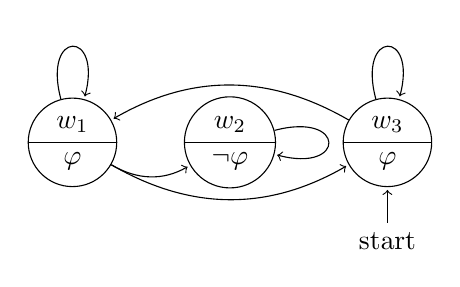
\begin{tikzpicture}[state/.style=state with output,shorten >=1pt,node distance=2cm,on grid,auto] 
   \node[state] (i_1)   {$w_1$ \nodepart{lower} $\varphi$}; 
   \node[state] (i_2) [right=of i_1] {$w_2$ \nodepart{lower} $\neg \varphi$}; 
   \node[state,initial below] (i_3) [right=of i_2] {$w_3$\nodepart{lower} $\varphi$}; 
    \path[->] 
    (i_1) edge [loop above] node {} ()
          edge [bend right] node {} (i_2) 
          edge [bend right] node {} (i_3) 
    (i_2) edge [loop right] node {} () 
    (i_3) edge [loop above] node {} () 
          edge [bend right] node {} (i_1);
\end{tikzpicture}
\end{minipage}
\begin{minipage}{.47\textwidth} 
\includegraphics[width=.95\textwidth]{isabelle/Counterexample2}
  %\caption{LogiKEy: Logic-pluralistic KR\&R}
  \label{fig:Counterexample1a}
  \end{minipage}
\end{figure}
\vskip-1em

%\noindent 
As prior work demonstrates, see e.g.~\cite{C47,IntuitionisticCube,J68} and also \cite{J40}, \texttt{nitpick} regularly provides intuitive and sometimes even surprising counterexamples when used in conjunction with shallow embeddings.\footnote{Prior work~\cite{C47,IntuitionisticCube} also illustrates how the counter-examples reported by \texttt{nitpick} could be systematically converted into statements that verifiably disprove the original conjecture in Isabelle/HOL; the pattern-based recipes presented there could indeed be fully automated.}  This is not only very useful in computer-supported logic education, but has also provided valuable feedback for research studies as reported, e.g.~in~\cite{J40}. However, some non-classical logics have only infinite models, and then the finite model finder \texttt{nitpick} is of no help; this is e.g.~the case for Lorini's T-STIT logic \cite{Lorini2013}, which was shallowly embedded by Meder \cite{MederMasters}.
The development of infinite model finding tools and their integration into proof assistants such as Isabelle/HOL is thus an important challenge for further research, as is the automated, domain- and application-adapted provision of intuitive counterexample diagrams to the user.

For further false conjectures (in lines 30-32), including modal collapse $\varphi \supset^m \Box^m \varphi$,  intuitive counterexamples are generated by \texttt{nitpick}. Finally, examples of simple modal theorems (in lines 34-35), such as the KB theorem $\Diamond^m \Box^m  \varphi \supset^m \Box^m \Diamond^m \varphi$, are automated efficiently using \texttt{smt} solvers in combination with definition unfolding in metalogic HOL.

\paragraph{Reasoning at object level.} 
Figure \ref{fig:PMLinHOL_shallow_minimal_further_tests} presents 
further proof experiments. After proving the schematic modal principle $K\Diamond$ (in line 5) an object level proof example \cite[Example 6.10]{Sider2009} is studied (in lines 8-16): $\Box^m P^m \supset^m (\Diamond^m Q^m \supset^m \Diamond^m (P^m \wedge^m Q^m))$, where $P$ and $Q$ are now propositional constant symbols in the PML signature $\mathcal{S}$. This statement is again effectively automated via definition unfolding at the metalevel HOL (line 8), while the presented interactive proof again uses the propositional Hilbert calculus from before in combination with the modal rule of necessitation, the distribution axiom of base modal logic $\mathbf{K}$ and the newly introduced \textbf{$K\Diamond$}-principle.
\begin{figure}[tp!]
  \centering
  \colorbox{gray!30}{\includegraphics[width=.97\textwidth]{isabelle/PMLinHOL_shallow_minimal_further_tests.png}}
  \caption{Experiments: Simple proof in modal logic \textbf{K}.}
  \label{fig:PMLinHOL_shallow_minimal_further_tests}
\end{figure}


Larger object-level proof examples could now be presented and studied using the minimal shallow embedding. Related studies have shown that the this approach is generally competitive, in particular, when it comes to reasoning in quantified modal logics; see e.g.~the recent experiments reported in \cite{J72}. Recipes for embedding modal quantifiers and extensive application studies for quantified modal logics are available in prior works; see e.g.~\cite{J23,J75}. 


\paragraph{Experiments with the Löb-axiom.} 
Figure~\ref{fig:PMLinHOL_shallow_minimal_Loeb_tests} presents automation experiments with the Löb-axiom of provability logic \cite{Boolos1994}. 
\begin{figure}[tp!]
  \centering
  \colorbox{gray!30}{\includegraphics[width=.97\textwidth]{isabelle/PMLinHOL_shallow_minimal_Loeb_tests.png}}
  \caption{Experiments: Studying the Löb-axiom of provability logic.}
  \label{fig:PMLinHOL_shallow_minimal_Loeb_tests}
\end{figure}
A first observation, interesting for education and research, 
is that via definition unfolding the schematic axioms are  automatically converted into corresponding formulas in metalogic HOL. For the Löb-axiom (in line 4) we thus obtain after definition unfolding the HOL formula $\forall \varphi\, w.\, (\forall v.\, \texttt{R} w v \longrightarrow (\forall z.\, \texttt{R} v z \longrightarrow \varphi z) \longrightarrow \varphi v) \longrightarrow (\forall v.\, \texttt{R} w v \longrightarrow \varphi v)$, as can be seen in the lower white window area of Isabelle/HOL displayed in Fig.~\ref{fig:PMLinHOL_shallow_minimal_Loeb_tests}. When using the maximal shallow embedding instead, the Löb-axiom unfolds into the expected much heavier HOL formula $\forall\varphi\, W R\, V\, x.\, W\, x \longrightarrow (\forall z.\, W\, z \longrightarrow R x z \longrightarrow (\forall x.\, W x \longrightarrow R z x \longrightarrow \varphi W R V x) \longrightarrow \varphi W R V z) \longrightarrow (\forall z.\, W z \longrightarrow R x z \longrightarrow \varphi W R V z)$, which also explains why automated reasoning is generally much harder for maximal shallow embeddings than for minimal shallow embeddings. Using such features of the presented framework, students are given the opportunity to e.g. explore frame properties for non-trivial properties on their own, to eventually simplify them and, using proof automation or interactive proof, to show them equivalent to already known properties, as also attempted in Fig.~\ref{fig:PMLinHOL_shallow_minimal_Loeb_tests} (in lines 5-9). As shown, such proof automation attempts succeed for the following conjectures: (line 5) the converse well-foundedness of the accessibility relation $\texttt{R}$ in combination with the transitivity of $\texttt{R}$ implies the Löb axiom, (line 7) the Löb axiom implies converse well-foundedness of  $\texttt{R}$, and (line 9) the Löb axiom implies the irreflexivity of $\texttt{R}$. Whenever transitivity is an implicant to be proved, proof automation still fails (see lines 6 and 8). Here interactive proof is needed or, alternatively, improved HOL theorem proving systems, in particular HOL provers that can suitably guess non-trivial instantiations for higher-order order variables as (apparently) required here.\footnote{For more on this challenge topic see e.g.~the experiments reported in~\cite{J63}.}

\paragraph{Performance.} The performance of $\texttt{sledgehammer}$ and $\texttt{nitpick}$ for the different embeddings is briefly discussed:\footnote{Of course, due to the relative simplicity of PML and the majority of test examples presented, these experiments are not yet conclusive. However, they provide evidence for the rationally expected result: The minimal shallow embedding performs better than the maximal shallow embedding and the deep embedding.}  
\emph{Minimal shallow embedding:} Proofs for 36 out of 38 valid statements (theorems, lemmas and substatements in interactive proofs) 
%as contained in Figs.\ref{fig:PMLinHOL_shallow_minimal_tests}-\ref{fig:PMLinHOL_shallow_minimal_Loeb_tests} 
were found by calls to $\texttt{sledgehammer}$.\footnote{A MacBook Air (Apple M3, 16GB memory, macOS 15.3.1) and Isabelle 2024 in its standard configuration was used, which sets a 60s prover timeout for $\texttt{sledgehammer}$. The response time was typically less than a second; except for the Löb tests. Theorems \texttt{Sound1} and \texttt{Sound2} were not counted.}
Nitpick reported counterexamples for 5 out of 5 invalid statements. Reconstruction of $\texttt{sledgehammer}$ proofs with trusted tactics failed in 2 cases. 
%
\emph{Maximal shallow embedding:} Proofs for 34 out of 38 valid statements were found by calls to $\texttt{sledgehammer}$.
Countermodels for 4 out of 5 invalid statements were found by nitpick. Reconstruction of $\texttt{sledgehammer}$ proofs with trusted tactics failed in 4 cases. 
%
\emph{Deep embedding:} Proofs for 33 out of 38 valid statements were found by calls to $\texttt{sledgehammer}$; in particular, there were no proofs delivered for the Löb examples.
Countermodels for 5 out of 5 invalid statements were found by nitpick. Reconstruction of $\texttt{sledgehammer}$ proofs with trusted tactics failed in 2 cases. 

% Tests: 
% PMLinHOL_shallow_minimal_tests: 
%     25 valid, 25 proved with sledgehammer
%     4 invalid, 4 counterexamples obtained with nitpick
% PMLinHOL_shallow_minimal_further_tests: 
%     8 valid, 8 proved with sledgehammer
% PMLinHOL_shallow_minimal_Loeb_tests
%     5 valid, 3 proved with sledgehammer
%     1 invalid, 1 counterexample obtained with nitpick



\section{Related work and implications for \logikey}
\label{sec:logikey}

Much related work on the connections between deep and shallow embeddings can actually be found in the literature, see e.g.~\cite{SvenningssonA12,KaposiKK19,PrinzKL22,WangCT24} and the references therein. However, there seems to be no work reported yet which achieved the automation of faithfulness proofs between deep and (different degrees of) shallow embeddings as demonstrated in this paper. 



\paragraph{Deep embeddings.}
Exemplary developments and applications of non-trivial deep logic embeddings include self-verifications of the HOL light logic \cite{Harrison06,AbrahamssonMKS22}, a formalization of the Core Why3 logic \cite{10.1145/3632902}, and a provably sound implementation of a differential dynamic logic \cite{deep2017}, to name a few. For examples of deep embeddings of logics and their calculi in the Coq proof assistant \cite{Coq}, see e.g.~\cite{SozeauABCFKMTW20} and the references therein, and Isabelle/HOL examples are presented in \cite{BlanchettePT17,FOL_Seq_Calc3-AFP,Implicational_Logic-AFP,LIPIcs.ITP.2022.13}. Further related work on the self-verification or bootstrapping of theorem provers 
can be found in \cite{Carneiro20}, and more recently in \cite{carneiro2024lean4leanverifiedtypecheckerlean} in the context of Lean \cite{Lean}.
% on deep embeddings in the proof assistant Lean \cite{Lean}.

\paragraph{Shallow embeddings.}
Exemplary work in this category, which Nipkow called the extensional approach \cite{Nipkow2002}, includes a mechanization of HOL reasoning in first-order set theory \cite{GuilloudGGK24}, the techniques presented in~\cite{KaposiKK19} to overcome some problems of shallow embedding for reasoning over the syntax of embedded languages, a shallow embedding for a pure type systems in first-order logic~\cite{LIPIcs.TYPES.2016.9}, and various other works such as~\cite{RabeLP14,LammichM12}; see also the references given in \cite{WangCT24}.
Moreover, note also that the automation support for various quantified non-classical logics as realized in the HOL theorem prover Leo3 \cite{J51,J72} is based on shallow embeddings. 


\paragraph{Implications for \logikey.}
The logic-pluralistic knowledge and reasoning methodology \logikey \cite{J48}, see Fig.~\ref{fig:LogiKEy}, leverages higher-order logic (HOL) as a unifying metalogic to enable the modeling of diverse object logics, so far,  primarily via using shallow semantic embeddings. 

\logikey\ has been used in a number of application domains and contexts where different object logics, such as free logic or modal higher-order logic, for example, have been used as a starting point; see e.g.~\cite{J40,J75,J68} 

This paper illustrates how the \logikey approach may benefit in the future from systematically provided, mutually faithful deep and shallow embeddings of all its supported object logics, so that they be used interchangeably. 
The technique presented in this paper has also the potential to replace or complement many pen and paper proofs to establish faithfulness results in prior works, such as e.g.~given in \cite{J23,J31,J58}, by verified proofs within the proof assistant. This in turn will be relevant for enabling applications in areas that require highest levels of trust. For this note that a particular application direction of \logikey\ is normative and legal reasoning in the context of AI regulation, see also \cite{R93}.

Moreover, with respect to the \logikey\ context, this paper also illustrates the conceptual changes that were applied in the transition in previous work from lightweight shallow embeddings of non-classical logics, as used for example for encoding higher-order modal logic \cite{J23} or conditional logic \cite{J31} (which take into account minimal dependencies on possible worlds only), to more heavyweight shallow embeddings, such as public announcement logic \cite{J58}, in which additional dependencies (on evaluation domains) had to be maintained. In prior work the explicit modeling of atoms, signatures and valuations was also often avoided.

Most importantly, the presented technique for linking deep and shallow embeddings will be very fruitful for furthering the use of \logikey\ in university-level logic courses, including in particular the author's courses on universal logical reasoning that have been taught at the Free University of Berlin and now at the University of Bamberg for the last decade.


\tikzset{block/.style={draw, thick, text width=2cm, minimum height=1.3cm, align=center}, 
         line/.style={-latex} }
\tikzset{ font={\fontsize{12pt}{12}\selectfont}}

\tikzset{testpic1/.pic={ 
\node[block, fill=green!20, text width=10cm, minimum width=14cm, minimum height=2cm] (m1) 
      { \textbf{\huge L3 --- Applications} };
\node[block, below=.5cm of m1, fill=orange!30, text width=14cm, minimum height=2cm] (m2) 
      { \textbf{\huge L2 --- Domain-Specific Language(s)} };
\node[block, below=.5cm of m2, fill=yellow!20, text width=10cm, minimum width=14cm, minimum height=2cm] (m3) 
      { \textbf{\huge L1 --- Object Logic(s)} };
\node[block, below=.5cm of m3, fill=blue!20, text width=11cm, minimum width=14cm, minimum height=2cm] (m4) 
      { \textbf{\huge L0 --- Meta-Logic (HOL)} };
\node[block, above right=-.5cm and 1.5cm of m1, fill=gray!40, text width=8cm, minimum width=9cm, minimum height=2cm, rotate=-90] (r1) 
      { \textbf{\huge \logikey\ Methodology} };

  \begin{scope}[on background layer] 
    \node[draw, fill=blue!20, inner xsep=5mm, inner ysep=5mm, fill opacity=0.6, fit=(m1)(m2)(m3)(m4)](m1tom4){};
  \end{scope}

  \begin{scope}[on background layer] 
    \node[draw, fill=gray!40, inner xsep=20mm, inner ysep=5mm, fill opacity=0.5, fit=(m1)(m2)(m3)(m4)(m1tom4)](all){};
  \end{scope}
}}


\tikzset{testpic2/.pic={ 
\node[block, fill=green!20, text width=10cm, minimum width=14cm, minimum height=2cm] (m1) 
      { \mbox{\textbf{\huge Gödel's Ontological Argument}} };
\node[block, below=.5cm of m1, fill=orange!30, text width=14cm, minimum height=2cm] (m2) 
      { \textbf{\huge Theory of Positive Properties} };
\node[block, below=.5cm of m2, fill=yellow!20, text width=10cm, minimum width=14cm, minimum height=2cm] (m3) 
      { \textbf{\huge Higher-Order Modal Logic} };
\node[block, below=.5cm of m3, fill=blue!20, text width=11cm, minimum width=14cm, minimum height=2cm] (m4) 
      { \textbf{\huge Meta-Logic (HOL)} };

  \begin{scope}[on background layer] 
    \node[draw, fill=blue!20, inner xsep=5mm, inner ysep=5mm, fill opacity=0.6, fit=(m1)(m2)(m3)(m4)](m1tom4){};
  \end{scope}
}}

\tikzset{testpic3/.pic={ 
\node[block, fill=green!20, text width=10cm, minimum width=14cm, minimum height=2cm] (m1) 
      { \mbox{\textbf{\huge Wise Men Puzzle}} };
\node[block, below=.5cm of m1, fill=orange!30, text width=14cm, minimum height=2cm] (m2) 
      { \textbf{\huge Theory of Agent(s) Knowledge} };
\node[block, below=.5cm of m2, fill=yellow!20, text width=10cm, minimum width=14cm, minimum height=2cm] (m3) 
      { \textbf{\huge Public Announcement Logic} };
\node[block, below=.5cm of m3, fill=blue!20, text width=11cm, minimum width=14cm, minimum height=2cm] (m4) 
      { \textbf{\huge Meta-Logic (HOL)} };

  \begin{scope}[on background layer] 
    \node[draw, fill=blue!20, inner xsep=5mm, inner ysep=5mm, fill opacity=0.6, fit=(m1)(m2)(m3)(m4)](m1tom4){};
  \end{scope}
}}

\begin{figure}[tp!]
\centering 
\begin{minipage}{.70\textwidth}
\resizebox{\textwidth}{!}{
    \begin{tikzpicture}
      \pic{testpic1};
    \end{tikzpicture}
    }
\end{minipage}
\hfill
\begin{minipage}{.28\textwidth}
\resizebox{\textwidth}{!}{
    \begin{tikzpicture}
      \pic{testpic2};
    \end{tikzpicture}
    }
\vskip.3em
\resizebox{\textwidth}{!}{    
    \begin{tikzpicture}
      \pic{testpic3};
    \end{tikzpicture} 
    }
\end{minipage}
\caption{The logic-pluralistic knowledge representation and reasoning methodology \logikey (left) and two concrete applications of it (right): Studies on Gödel's ontological argument \cite{J75} (top) and an automation of the wise men puzzle \cite{J58} (bottom). \label{fig:LogiKEy}}
\end{figure}


\section{Conclusion}
\label{sec:conclusion}
This paper has shown how interlinked deep and (varying degrees of) shallow logic embeddings can be modeled and implemented in classical higher-order logic, as provided by many modern proof-assistant systems. This technique allows for the mechanization of faithfulness proofs between these embeddings, and, as has been shown in this paper, can even support the automation of such proofs. 

The presented technique is interesting for future research in several ways, and is particularly suited to support logic education due to its conciseness, elegance, and support for interactive and automated theorem proving and counterexample finding. The latter was a motivation to illustrate the approach in this paper using simple propositional modal logic, which is routinely used as introductory material in logic courses worldwide. The provided Isabelle/HOL sources should be easily reusable in such a context, and only some basic features of Isabelle/HOL have been used to additionally support this idea.  

\subsubsection{Acknowledgements}
Thanks are due to all the \logikey contributors over the past ten to fifteen years.


% ---- Bibliography ----
%
% BibTeX users should specify bibliography style 'splncs04'.
% References will then be sorted and formatted in the correct style.
%
\bibliographystyle{splncs04}
\bibliography{chris,literature}

%\printbibliography

\newpage
\begin{appendix}
\section{Preliminaries}
\label{sec:preliminaries}
Figure~\ref{fig:Preliminaries} presents preliminaries that are uniform for all embeddings studied and which are imported by all Isabelle/HOL theory files presented in this paper. 

Two HOL base types $\texttt{w}$ and $\mathcal{S}$ are declared (in lines 4-5) to denote a (nonempty) set of possible worlds and a (nonempty) set of propositional constant symbols, the signature common to all embeddings discussed in this paper. Then (in line 6) the exemplary signature  symbols $\texttt{p}$, $\texttt{p}$ and $\texttt{r}$ are introduced, and type synonyms are declared (in lines 7-8): $\mathcal{W}$ for sets of possible worlds (universe), $\mathcal{R}$ for binary relations on $W$ (accessibility relations), and
$\mathcal{V}$ for evaluation functions that assign truth values to the symbols $a \in \mathcal{S}$ for each world $w$. Then some well-known relational properties are introduced as abbreviations (in lines 11-19), and the guarded quantifier notation $\forall w{:}W.\, \varphi$ is defined to stand for $\forall w. \,W\,w \longrightarrow \varphi$ ($W$ is of type $\mathcal{W}$). Finally, the useful backward implication $\longleftarrow$ is defined, which is unfortunately missing in Isabelle/HOL.

\begin{figure}[!ht]
  \centering
  \colorbox{gray!30}{\includegraphics[width=.97\textwidth]{isabelle/PMLinHOL_preliminaries.png}}
  \caption{Preliminaries.}
  \label{fig:Preliminaries}
\end{figure}

\section{Alternative experiments}
\label{sec:alternative_experiments}
Experiments with the maximal shallow embedding 
and the deep embedding of PML in HOL 
are presented in Figs.~\ref{fig:PMLinHOL_shallow} and ~\ref{fig:PMLinHOL_deep} respectively. Automation results that divert from those reported for the minimal shallow embedding are highlighted by $\textcolor{red}{(**)}$.
\newpage

\begin{figure}[htp!]
  \centering
  \colorbox{gray!30}{\includegraphics[width=.97\textwidth]{isabelle/PMLinHOL_shallow_tests.png}}
   \vskip.5em
  \colorbox{gray!30}{\includegraphics[width=.97\textwidth]{isabelle/PMLinHOL_shallow_further_tests}}
   \vskip.5em
  \colorbox{gray!30}{\includegraphics[width=.97\textwidth]{isabelle/PMLinHOL_shallow_Loeb_tests}}
  \caption{Experiments with the maximal shallow embedding of PML in HOL. \label{fig:PMLinHOL_shallow}}
\end{figure}

\newpage
\begin{figure}[htp!]
  \centering
  \colorbox{gray!30}{\includegraphics[width=.97\textwidth]{isabelle/PMLinHOL_deep_tests.png}}
  \vskip.5em
  \colorbox{gray!30}{\includegraphics[width=.97\textwidth]{isabelle/PMLinHOL_deep_further_tests}}
   \vskip.5em
  \colorbox{gray!30}{\includegraphics[width=.97\textwidth]{isabelle/PMLinHOL_deep_Loeb_tests}}
  \caption{Experiments with the deep embedding of PML in HOL. \label{fig:PMLinHOL_deep}}
\end{figure}



\end{appendix}
\end{document}
